\documentclass[tikz]{standalone}

\begin{document}
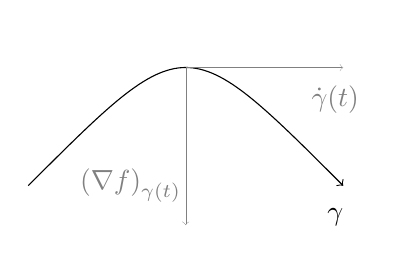
\begin{tikzpicture}[scale=2]
  \draw[->] 
  (0, 0) .. controls +(1, 1) and +(-1, 1)
  .. (2, 0);
  \node at (1.95, -0.2) {$\gamma$};
  \draw[gray, ->, ultra thin] (1, 0.75) -- (2, 0.75);
  \draw[gray, ->, ultra thin] (1, 0.75) -- (1, -0.25);
  \node[gray] at (1.95, 0.55) {$\dot \gamma(t)$};
  \node[gray] at (0.65, -0) {${(\nabla f)}_{\gamma(t)}$};
  
\end{tikzpicture}
\end{document}
